% ShiftWM architecture figure (vector + real-data insets from arch_assets.py).
% Build: tectonic architecture.tex && cp architecture.pdf ../architecture.pdf
\documentclass[tikz,border=3pt]{standalone}
\usepackage[T1]{fontenc}
\usepackage[scaled=0.92]{helvet}
\renewcommand{\familydefault}{\sfdefault}
\usepackage{amsmath,amssymb,bm}
\usetikzlibrary{arrows.meta,positioning,calc,backgrounds,shadows,fit}
\definecolor{ink}{HTML}{1F2A37}
\definecolor{subink}{HTML}{5B6573}
\definecolor{obsblue}{HTML}{0072B2}
\definecolor{dynorange}{HTML}{D55E00}
\definecolor{oursgreen}{HTML}{009E73}
\definecolor{actpurple}{HTML}{7B4FA0}
\definecolor{frozen}{HTML}{EEF1F5}
\newcommand{\Z}{\mathbf{Z}}
\newcommand{\h}{\mathbf{h}}
\tikzset{
  >={Stealth[length=2.3mm,width=1.7mm]},
  card/.style={draw=#1!55, line width=0.7pt, fill=white, rounded corners=4pt,
               drop shadow={opacity=0.13, shadow xshift=0.7pt, shadow yshift=-0.9pt}},
  flow/.style={->, line width=1.05pt, draw=ink!80, rounded corners=5pt},
  actflow/.style={->, line width=1.0pt, draw=actpurple!85, rounded corners=5pt},
  obsflow/.style={line width=1.1pt, draw=obsblue, dash pattern=on 3.5pt off 2pt, rounded corners=6pt},
  title/.style={font=\bfseries\small, text=ink},
  sub/.style={font=\scriptsize, text=subink, align=center},
  stage/.style={font=\bfseries\footnotesize, text=#1!80!black},
  chip/.style={draw=actpurple!60, fill=actpurple!9, rounded corners=2pt, minimum width=0.66cm,
               minimum height=0.44cm, inner sep=1pt, font=\scriptsize, text=ink},
}
% stacked layer block: #1 name, #2 centre, #3 width, #4 height, #5 colour
\newcommand{\layerstack}[5]{%
  \fill[#5!10, rounded corners=4pt] ($#2+(-#3/2+0.16,-#4/2+0.16)$) rectangle ($#2+(#3/2+0.16,#4/2+0.16)$);
  \draw[#5!35, rounded corners=4pt, line width=0.5pt] ($#2+(-#3/2+0.16,-#4/2+0.16)$) rectangle ($#2+(#3/2+0.16,#4/2+0.16)$);
  \fill[#5!14, rounded corners=4pt] ($#2+(-#3/2+0.08,-#4/2+0.08)$) rectangle ($#2+(#3/2+0.08,#4/2+0.08)$);
  \draw[#5!45, rounded corners=4pt, line width=0.5pt] ($#2+(-#3/2+0.08,-#4/2+0.08)$) rectangle ($#2+(#3/2+0.08,#4/2+0.08)$);
  \node[card=#5, minimum width=#3 cm, minimum height=#4 cm] (#1) at #2 {};}
% token grid tile: #1 origin, #2 size, #3 colour
\newcommand{\tokentile}[3]{%
  \begin{scope}[shift={#1}]
    \fill[#3, rounded corners=1.5pt] (0,0) rectangle (#2,#2);
    \draw[white, line width=0.3pt, step=#2/8] (0,0) grid (#2,#2);
    \draw[ink!45, line width=0.5pt, rounded corners=1.5pt] (0,0) rectangle (#2,#2);
  \end{scope}}
\newcommand{\stepbadge}[3]{\node[circle, fill=#1, text=white, font=\bfseries\scriptsize, inner sep=1.2pt, minimum size=0.42cm] at #2 {#3};}
\begin{document}
\begin{tikzpicture}[font=\sffamily]
% Designed at the ICLR text width (13.97 cm) so it is included at 100% scale.
\begin{scope}[on background layer]
  \fill[obsblue!5, rounded corners=7pt] (0,0) rectangle (3.15,5.3);
  \fill[dynorange!5, rounded corners=7pt] (3.3,0) rectangle (7.55,5.3);
  \fill[oursgreen!6, rounded corners=7pt] (7.7,0) rectangle (13.95,5.3);
\end{scope}
\stepbadge{obsblue}{(0.33,4.98)}{1}
\node[stage=obsblue, anchor=west] at (0.56,4.98) {Observe};
\stepbadge{dynorange}{(3.63,4.98)}{2}
\node[stage=dynorange, anchor=west] at (3.86,4.98) {Condition on actions};
\stepbadge{oursgreen}{(8.03,4.98)}{3}
\node[stage=oursgreen, anchor=west] at (8.26,4.98) {Move, then correct};

% ---------------------------------------------------------------- 1 observe
\foreach \dx in {0.16,0.08}{
  \fill[white, draw=subink!35, rounded corners=1pt, line width=0.4pt] (0.3+\dx,2.95+\dx) rectangle (2.75+\dx,4.33+\dx);}
\node[inner sep=0pt, drop shadow={opacity=0.2, shadow xshift=0.8pt, shadow yshift=-1pt}, anchor=south west]
  (img) at (0.3,2.95) {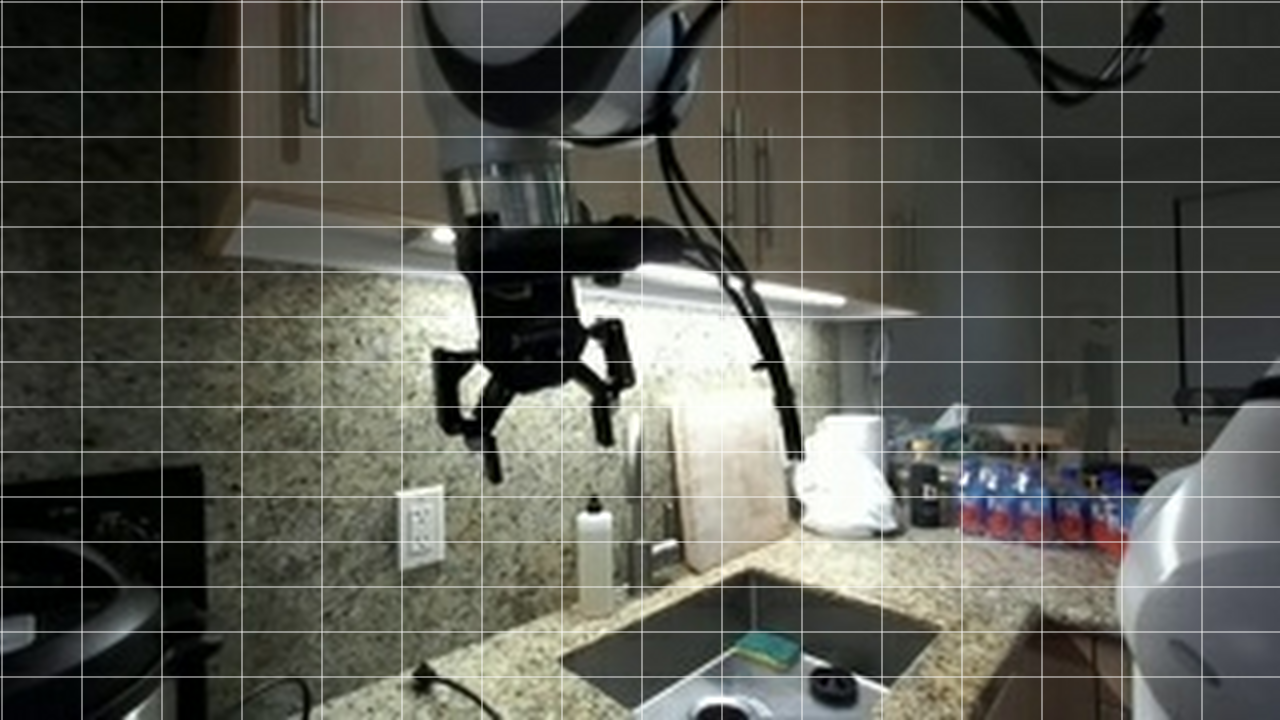
\includegraphics[width=2.45cm,height=1.38cm]{arch_assets/observed_2.png}};
\node[sub, anchor=north] at (img.south) {3 observed frames};
\node[draw=subink!40, fill=frozen, rounded corners=6pt, font=\scriptsize, text=ink, inner xsep=5pt, inner ysep=2.5pt]
  (enc) at (1.52,2.05) {frozen DINO encoder};
\draw[flow, draw=subink!70] ($(img.south)+(0,-0.3)$) -- (enc.north);
\foreach \i/\dx/\c in {0/0/obsblue!30,1/0.15/obsblue!48,2/0.3/obsblue!68}{
  \tokentile{(1.02+\dx,0.62-\dx+0.3)}{0.8}{\c}}
\draw[flow, draw=subink!70] (enc.south) -- (1.52,1.72);
\node[font=\scriptsize, text=ink, anchor=east] at (1.0,1.25) {$\Z_{-2:0}$};

% ---------------------------------------------------------------- 2 condition
\layerstack{mem}{(4.55,3.55)}{2.1}{1.25}{obsblue}
\node[title] at ($(mem.center)+(0,0.25)$) {Memory};
\node[sub] at ($(mem.center)+(0,-0.22)$) {space--time\\[-1pt]attention};
\layerstack{dec}{(6.5,3.55)}{1.75}{1.25}{dynorange}
\node[title] at ($(dec.center)+(0,0.25)$) {Decoder};
\node[sub] at ($(dec.center)+(0,-0.22)$) {queries for\\[-1pt]every $k$};
\draw[flow] (2.25,0.95) -- (3.55,0.95) |- (mem.west);
\draw[flow] (mem.east) -- (dec.west);

\foreach \j/\t in {0/{a_{<0}},1/{a_0},2/{\cdots},3/{a_{k-1}}}{
  \node[chip, minimum width=0.72cm, font=\scriptsize] (a\j) at (4.05+\j*0.86,0.72) {$\t$};}
\node[sub, anchor=north] at (5.35,0.44) {actions};
\draw[actflow] (a0.north) -- (a0.north |- mem.south);
\node[card=actpurple, minimum width=1.75cm, minimum height=0.7cm, font=\scriptsize\bfseries, text=ink] (gru) at (6.5,1.95) {causal GRU};
\draw[actflow] (a3.north) -- (a3.north |- gru.south);
\draw[actflow] (gru.north) -- node[right, font=\scriptsize, text=actpurple] {$\mathbf{c}_k$} (dec.south);

% ---------------------------------------------------------------- 3 move & correct
\draw[line width=1.05pt, draw=ink!80] (dec.east) -- node[above, font=\scriptsize, text=ink] {$\h_k$} (7.95,3.55);
\draw[line width=1.05pt, draw=ink!80] (7.95,3.9) -- (7.95,1.0);

% (a) transport: the visual centrepiece
\node[card=oursgreen, minimum width=3.6cm, minimum height=2.45cm, anchor=west] (tp) at (8.15,3.38) {};
\node[inner sep=0pt, anchor=north west] (tpimg) at ($(tp.north west)+(0.1,-0.4)$) {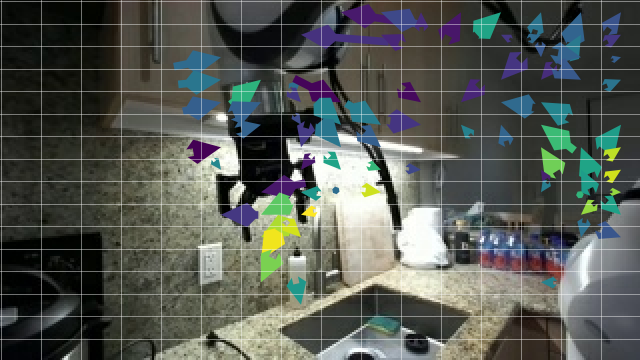
\includegraphics[width=3.4cm,height=1.95cm]{arch_assets/transport.png}};
\node[font=\footnotesize\bfseries, text=ink, anchor=north west] at ($(tp.north west)+(0.08,-0.03)$) {(a) transport of observed features};
\draw[flow] (7.95,3.9) -- ($(tp.west)+(0,0.55)$);

% (b) gate and (c) correction
\node[card=dynorange, minimum width=1.75cm, minimum height=1.42cm, anchor=north west] (gt) at (8.15,1.72) {};
\node[inner sep=0pt, anchor=north] (gtimg) at ($(gt.north)+(0,-0.1)$) {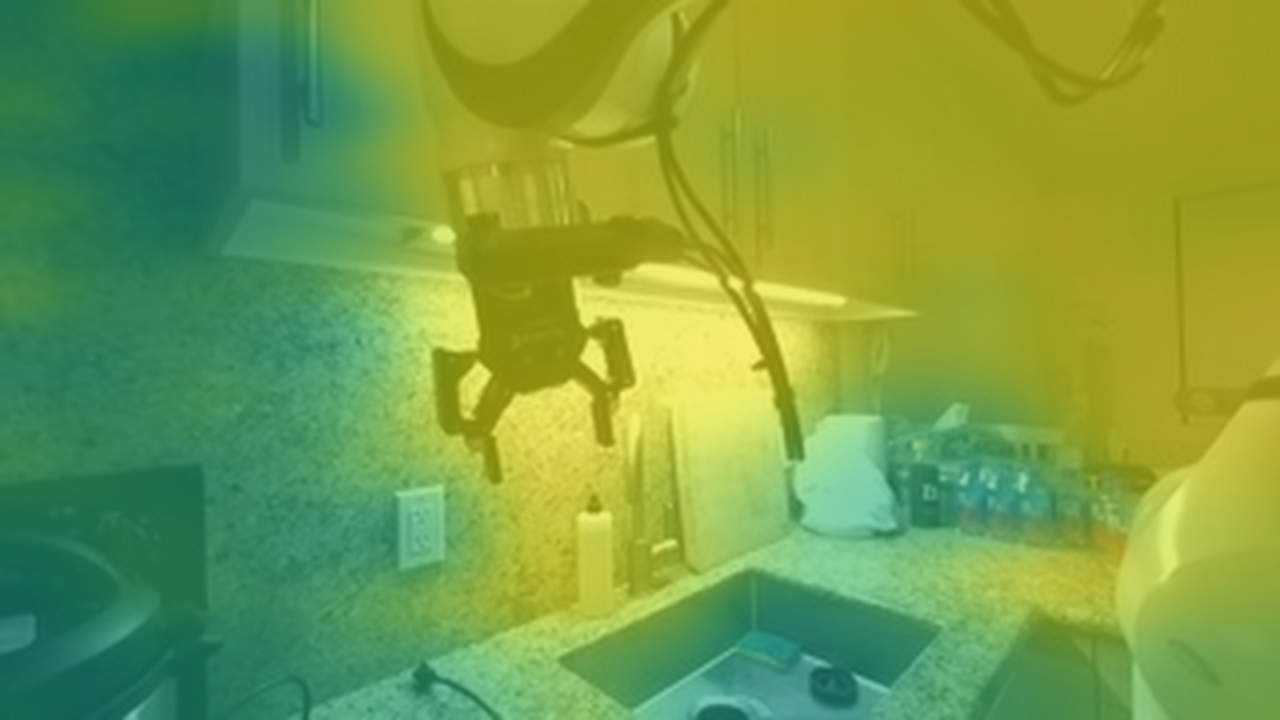
\includegraphics[width=1.55cm,height=0.87cm]{arch_assets/gate.png}};
\node[font=\scriptsize\bfseries, text=ink, anchor=south] at ($(gt.south)+(0,0.04)$) {(b) gate $g_k$};
\node[card=subink, minimum width=1.75cm, minimum height=1.42cm, anchor=north west, align=center, font=\scriptsize] (cr) at (10.0,1.72)
  {\bfseries (c) correction\\[3pt]\mdseries$\mathbf{r}_k$\\[-1pt]\color{subink}new content};
\draw[flow] (7.95,1.0) -- (gt.west |- 7.95,1.0);

% combine
\node[circle, draw=oursgreen!70!black, fill=white, line width=1pt, minimum size=0.6cm, inner sep=0pt,
      drop shadow={opacity=0.15, shadow xshift=0.6pt, shadow yshift=-0.7pt}, font=\large\bfseries, text=oursgreen!70!black] (plus) at (12.35,2.4) {$+$};
\draw[flow] (tp.east) -| (plus.north);
\draw[flow] (gt.north) -- (gt.north |- 0,1.92) -- (12.35,1.92) -- (plus.south);
\draw[flow] (cr.east) -| ($(plus.south east)+(0.05,-0.02)$);
\foreach \i/\dx/\c in {0/0/oursgreen!35,1/0.14/oursgreen!52,2/0.28/oursgreen!72}{
  \tokentile{(12.95+\dx,2.1-\dx)}{0.7}{\c}}
\node[font=\scriptsize\bfseries, text=ink, anchor=south] at (13.45,2.85) {$\hat\Z_{1..K}$};
\draw[flow] (plus.east) -- (12.93,2.4);
\node[draw=oursgreen!60!black, fill=oursgreen!10, rounded corners=4pt, line width=0.8pt, inner xsep=5pt, inner ysep=3pt,
      font=\scriptsize, text=ink, align=center] (eq) at (12.75,4.93) {$\hat\Z_k=(1-g_k)\,\Z_0$\\$+\,g_k\,\mathbf{T}_k+\mathbf{r}_k$};

% anchor path
\draw[obsflow, ->] (1.02,0.62) -- (0.2,0.62) -- (0.2,0.18) -- (13.1,0.18) -- node[right, font=\scriptsize\bfseries, text=obsblue] {$\Z_0$} (13.1,1.3);
\node[font=\scriptsize\bfseries, text=obsblue, fill=white, rounded corners=2pt, inner sep=1.5pt] at (6.2,0.18)
  {observed features are reused at every horizon --- never the model's own forecast};
\end{tikzpicture}
\end{document}
